\chapter{Interfaz gráfica de usuario}
\label{chap:GUI}
\Abstract{En este anexo se va a explicar el proceso de desarrollo de una interfaz gráfica de usuario desarrollada con MATLAB para el control del robot y las redes neuronales.}

Para facilitar el control del sistema y mejorar la interacción con el robot, se ha desarrollado una interfaz gráfica que permita a un usuario sin conocimientos de MATLAB, de redes neuronales o del robot, ser capaz de controlarlo. Esta interfaz ha sido desarrollado con la ayuda de App Designer de MATLAB (ver \autoref{fig:GUI app designer}). Se trata de una herramienta de MATLAB que facilita el desarrollo de interfaces gráficas de forma visual y sencilla, aunque también permite un mayor control a través de código.

\begin{figure}[ht]  %App designer
	\centering
	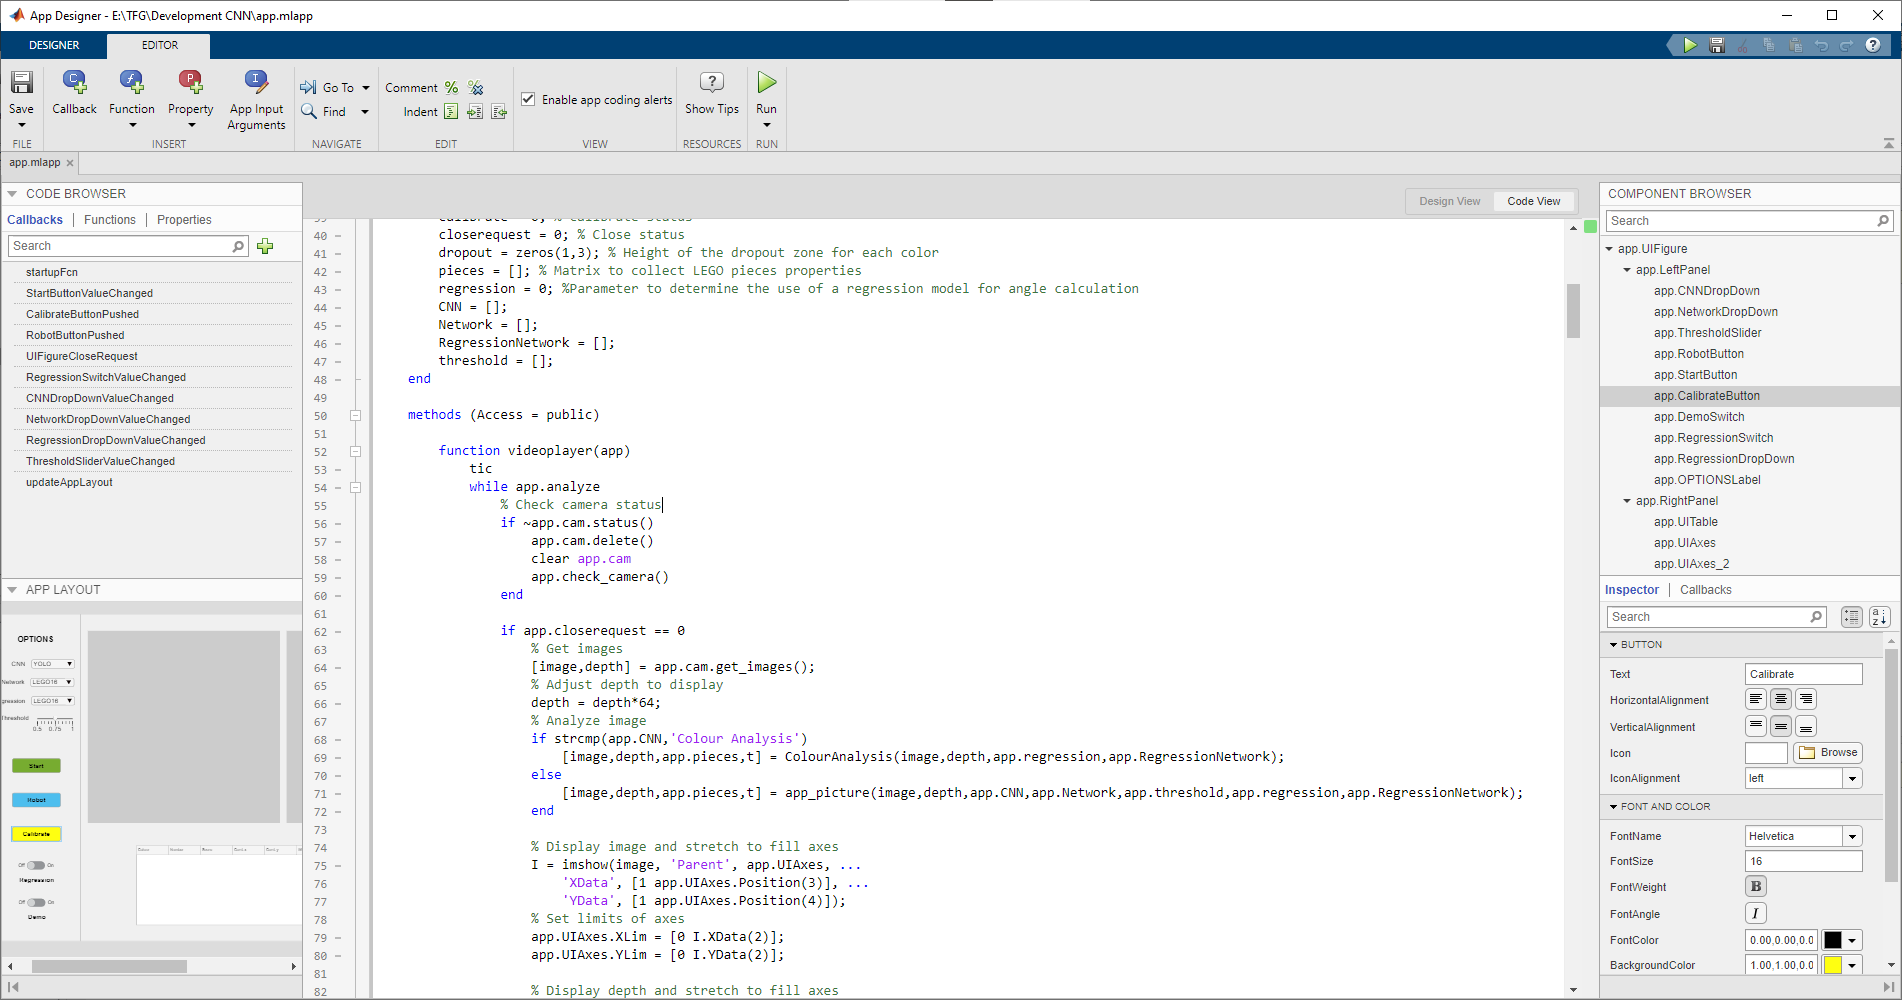
\includegraphics[width=0.95\textwidth]{Interfaz grafica de usuario/app designer.png}
	\caption{Desarrollo de una interfaz gráfica con App Designer}
	\label{fig:GUI app designer}
\end{figure}

\section{Interfaz}
La interfaz se ha decidido dividir en dos secciones para facilitar el manejo. La sección izquierda es la zona de control en la que el usuario puede determinar las opciones que desea emplear. Y la sección de la derecha es la zona en la que el programa muestra toda la información obtenida y los resultados del proceso de segmentación.

\begin{figure}[ht]  %Arranque
	\centering
	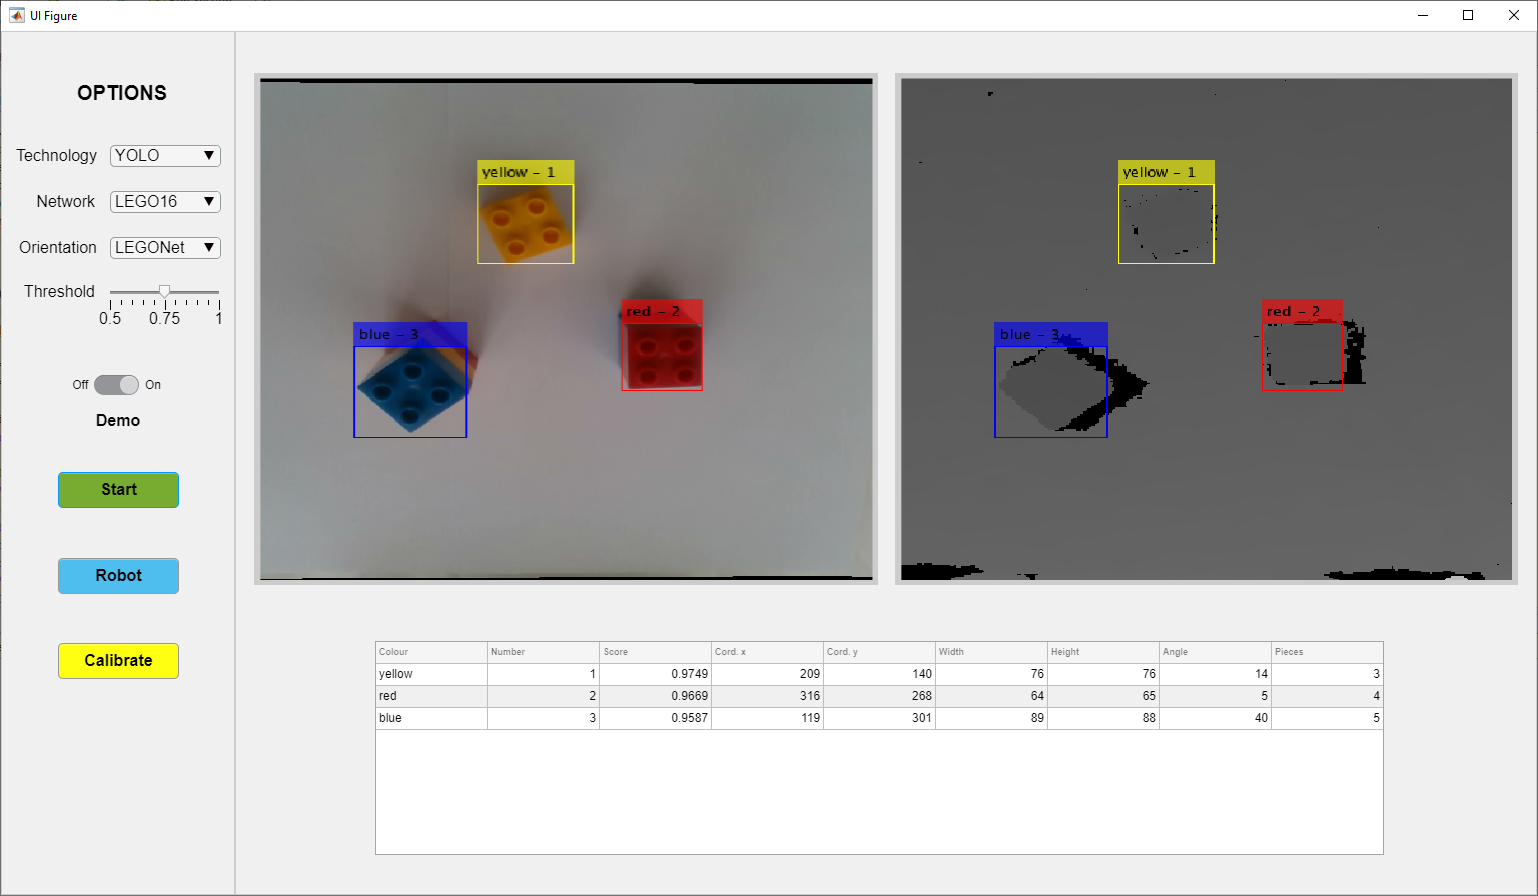
\includegraphics[width=0.95\textwidth]{Interfaz grafica de usuario/Arranque.png}
	\caption{Interfaz gráfica desarrollada con MATLAB}
	\label{fig:GUI arranque}
\end{figure}

\section{Controles}
Para facilitar el control y manejo del sistema se ha decidido que la interfaz sea fácil de usar y de entender, es por ello que son pocos los controles y opciones. Las opciones principales se dividen en tres categorías:

\begin{itemize}
\item Technology: Menú desplegable con el que se permite elegir que tipo de tecnología se desea emplear para el proceso de segmentación. Existen cuatro opciones entre las que elegir: YOLO, R-CNN, Faster R-CNN y Colour Analysis. Esta última se trata de la segmentación con máscaras de color desarrollada en \autoref{chap:Segmentacion con mascaras de color}.
\item Network: Menú desplegable con el que se permite elegir qué tipo de red neuronales se desea emplear para el proceso de segmentación. En caso de haber escogido algún tipo de tecnología basada en redes neuronales, esta opción determina el tipo de red con la que se desea trabajar. Es decir, da la opción de escoger entre LEGONet y LEGO16.
\item Orientatoin: Menú desplegable con el que se permite elegir qué tipo de tecnología se desea emplear para el proceso de cálculo de la rotación. Se permite escoger entre tres opciones, dos modelos de regressión basados en las redes neuronales LEGONet y LEGO16 y un sistema basado en la transformada de Hough.
\item Threshold: Control deslizante para ajustar el valor umbral de confianza para las redes neuronales.
\item Demo: Botón de activación para desconectar la conexión con el brazo robótico. Con el fin de poder simular el comportamiento del programa con el brazo robótico, se ha diseñado este botón que permite realizar todo a excepción de la conexión con el robot. De esta forma se puede ver el proceso del cálculo de coordenadas respecto al brazo robótico.
\item Start: Arranca el programa con los ajustes seleccionados en Technology, Network, Orientation y Threshold. Analiza de forma continua las imágenes recibidas por la cámara y muestra el resultado a través de la interfaz gráfica.
\item Robot: Manda las coordenadas obtenidas de la última imagen analiza al robot.
\item Calibrate: Permite recalibrar el mapa de profundidad para determinar la altura de las piezas.
\end{itemize}

\section{Medidas de seguridad}
Con el fin de ofrecer la mejor experiencia de usuario posible, se ha desarrollado varios sistemas de seguridad que comprueban constantemente el correcto funcionamiento del programa y la correcta conexión entre los diferentes dispositivos. Estas medidas de seguridad se pueden dividir en dos categorías:

\begin{itemize}
\item Comprobación de conexiones: El programa ha sido diseñado para asegurar de que en caso de que alguna conexión falle con el brazo robótico o la cámara, este sea capaz de recuperarse y continuar trabajando. Para ello antes de comunicarse con cualquiera de estos dispositivos primero comprueba su estado. El proceso es bastante rápido por lo que no perjudica mucho el rendimiento del programa.
\item Comunicación entre procesos: El sistema es capaz de realizar varios procesos de forma simultanea, pero esto puede suponer un problema ya que se pueden quedar procesos en cola que no puedan llegar a correrse nunca o que para cuando se intente correr el sistema ya no este preparado para correrlos. Es por eso por lo que se ha diseñado un sistema de control que evita que los procesos se almacenen o interrumpan entre si cuando no es debido,
\end{itemize}

\section{Problemas causados por la interfaz}
Una de las mayores carencias de MATLAB como lenguaje de programación es la falta de control sobre los hilos de ejecución. Durante el desarrollo de este proyecto esto no ha supuesto ningún problema ya que todo el proceso es bastante lineal y directo. Sin embargo, al desarrollar la interfaz se ha visto como el rendimiento del sistema ha reducido bastante ya que no puede separar la carga por hilos y hay múltiples sistemas que interrumpen constantemente la ejecución principal para hacer comprobaciones o actualizar valores. Si se trabaja con otro lenguaje de programación es muy probable que este problema pueda ser solventado.